% !TEX program = lualatex
\documentclass[10pt, aspectratio=169]{beamer}

\usepackage{appendixnumberbeamer}
\usepackage[export]{adjustbox}
\usepackage{booktabs}
\usepackage[scale=2]{ccicons}
\usepackage{pgfplots}
\usepackage{xspace}
\usepackage[compat=1.1.0]{tikz-feynman}

\usetheme[progressbar=frametitle,
subsectionpage=progressbar,
block=fill]{metropolis}

% make progress bar for every slide rather than just sections
\makeatletter
\setlength{\metropolis@frametitle@padding}{1.8ex}% <- default 2.2 ex
\setbeamertemplate{frametitle}{%
    \nointerlineskip%
    \begin{beamercolorbox}[%
        wd=\paperwidth,%
        sep=0pt,%
        leftskip=\metropolis@frametitle@padding,%
        rightskip=\metropolis@frametitle@padding,%
        ]{frametitle}%
        \metropolis@frametitlestrut@start%
        \insertframetitle%
        \nolinebreak%
        \metropolis@frametitlestrut@end%
    \end{beamercolorbox}
    \usebeamertemplate*{progress bar in head/foot}
}
\setlength{\metropolis@progressinheadfoot@linewidth}{1pt}



\usepgfplotslibrary{dateplot}

\newcommand{\themename}{\textbf{\textsc{metropolis}}\xspace}

\title{\Huge \textnormal{Improving Background Estimation for Di-Higgs Searches with ATLAS}}
\subtitle{PHYS 437B Presentations\newline
13 January, 2020}
% \date{\today}
\date{}
\author{Callum McCracken\\
Supervisor: Maximilian Swiatlowski\\
Co-Supervisor: Eduardo Martin-Martinez\\
Collaborators: Todd Seiss, Mel Shochet}

%\titlegraphic{\hfill\includegraphics[height=1.5cm]{logo.pdf}}
\setbeamercolor{background canvas}{bg=white}

\begin{document}

\maketitle

%%%%%%%%%%%%%%%%%%%%% SLIDE 1
{\setbeamertemplate{frame footer}{Image sources:
  \href{https://public-archive.web.cern.ch/en/research/AccelComplex-en.html}{\alert{Accelerator Complex}}, 
  \href{https://atlas.cern/discover/detector}{\alert{ATLAS}}, 
  \href{https://en.wikipedia.org/wiki/Higgs_boson}{\alert{Standard Model}}}
\begin{frame}{Overview: Higgs Research with ATLAS}
  \begin{columns}[onlytextwidth]
    \begin{column}{0.4\textwidth}
      \centering
      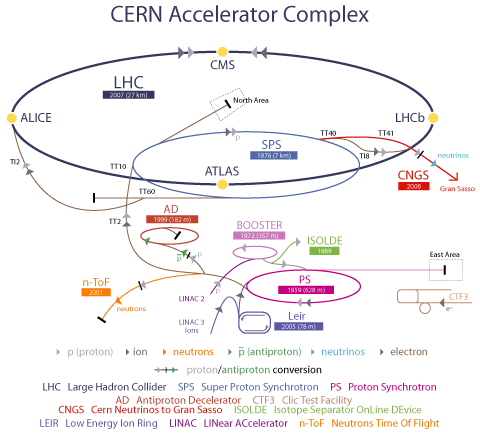
\includegraphics[width=0.9\linewidth]{images/accelerator_complex.png}
      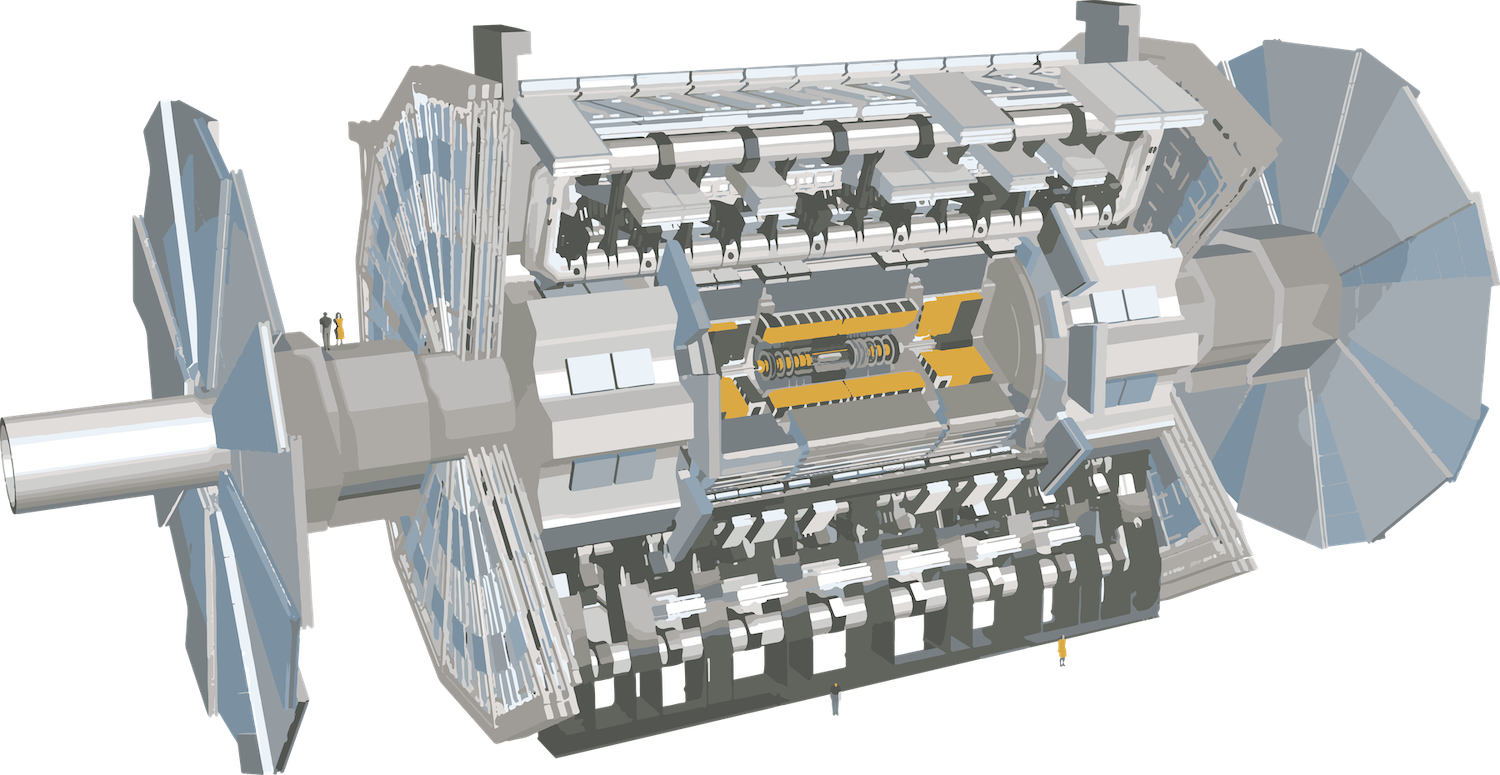
\includegraphics[width=0.9\linewidth]{images/ATLAS_full.png}
    \end{column}
    \begin{column}{0.6\textwidth}
      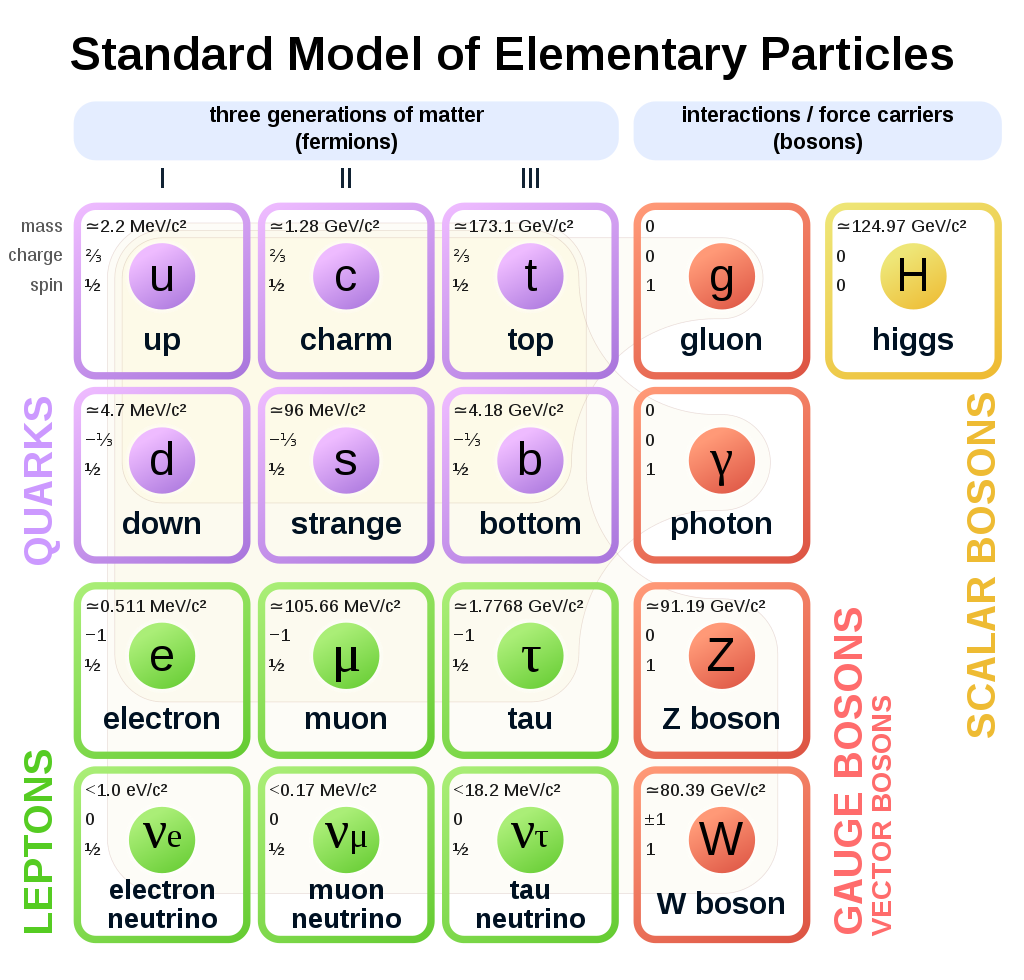
\includegraphics[width=0.9\linewidth]{images/Standard_Model_of_Elementary_Particles.png}
    \end{column}
​  \end{columns}
\end{frame}
}


%%%%%%%%%%%%%%%%%%%%% SLIDE 2
\begin{frame}{The Larger Project: Measuring the Higgs Self-Coupling}
  Relevant section of the SM Lagrangian for Higgs potential:\\
  
  $$V(\phi) = -\mu^2 \phi^2 + \lambda \phi^4 + \ldots \text{ Taylor exp. at min } \to V_T(\phi) = -\frac{\mu^4}{4\lambda} + \frac{\sqrt{2}\mu^3}{\lambda} \phi - 4 \mu^2\phi^2 + 2\sqrt{2\lambda}\mu\phi^3 + \ldots$$
  
  Constant and $\phi$ terms: can eliminate with change of coordinates, $\phi^2$: mass term,\\
  $\phi^3$: self-interaction or \alert{self-coupling} term, not well constrained\\ (current best: $\kappa_\lambda = (2\sqrt{2\lambda}\mu)/(2\sqrt{2\lambda}\mu)_{\text{SM}}$, $\kappa_\lambda \in [-2.3, 10.3]$ at 95\% confidence)

  \begin{center}
    \raisebox{3.5mm}{
    \feynmandiagram [small,horizontal=a to b] {
    i1 [particle=\($g$\)]
        -- [gluon] t1 [dot]
        --  [anti fermion] a [dot]
        --  [anti fermion] t2 [dot]
        -- [anti fermion, edge label=\($t/b$\) ] t1,
    t2 -- [gluon] i2 [particle=\($g$\)],
    i1 -- [opacity=0] i2,
    a [label=\(\kappa_t\)] -- [scalar, edge label'=\($H$\)] b [dot, label=\(\kappa_\lambda\)],
    f1 [particle=\($H$\)] -- [scalar] b -- [scalar] f2 [particle=\($H$\)] -- [opacity=0] f1,
    };}
\hspace{1cm}
    \feynmandiagram [small, layered layout, horizontal=a to b] {
    % Draw the top and bottom lines
    i1 [particle=\($g$\)]
    -- [gluon] a [dot]
    -- [fermion] b [dot, label=\(\kappa_t\)]
    -- [scalar] f1 [particle=\($H$\)],
    i2 [particle=\($g$\)]
   -- [gluon] c [dot]
    -- [anti fermion] d [dot, label=below:\(\kappa_t\)]
    -- [scalar] f2 [particle=\($H$\)],
    % Draw the two internal fermion lines
    { [same layer] a -- [anti fermion, edge label=\($t/b$\)] c },
    { [same layer] b -- [fermion] d},
    };
\end{center}

  To find $\kappa_\lambda$ we need $HH$ events, and we can find them using jets!
\end{frame}


%%%%%%%%%%%%%%%%%%%%% SLIDE 3
{\setbeamertemplate{frame footer}{Image sources: \href{https://arxiv.org/abs/1709.04533}{\alert{branching ratios}}, \href{https://en.wikipedia.org/wiki/B-tagging}{b-tagging image adapted from \alert{here}}}
\begin{frame}{Background: Jets and Pairing}
  \begin{columns}[onlytextwidth]
    \begin{column}{0.76\textwidth}
      \centering
      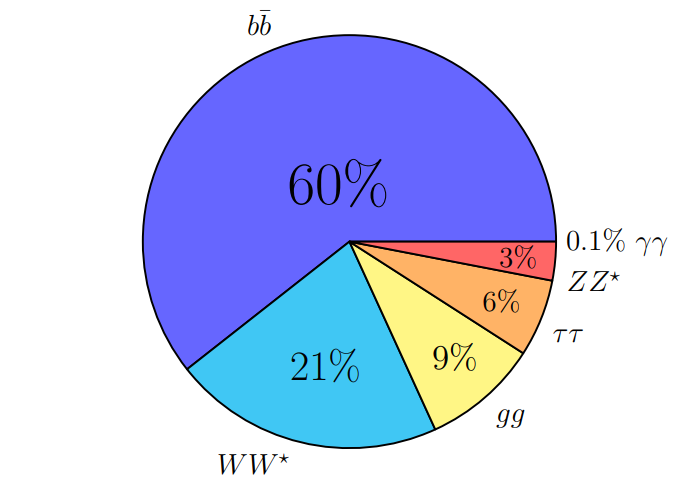
\includegraphics[width=0.35\linewidth]{images/branching_ratios.png}\\
      $H \to 60\%\space b\bar{b} \to 2 \times b \text{ hadrons } \to 2 \times b\text{-jets}$
      \begin{itemize}
        \item \alert{Jets} are collections of particles with appx. the same direction
        \item ATLAS can't directly detect $H$ or $b$. Instead, use \alert{$b$-jets}, which can be directly detected (using secondary vertices)
        \item $b$-jet detection is not a perfect process (hence 437A report), and neither is \alert{pairing} -- identifying which jets came from which $H$
      \end{itemize}
    \end{column}
    \begin{column}{0.25\textwidth}
      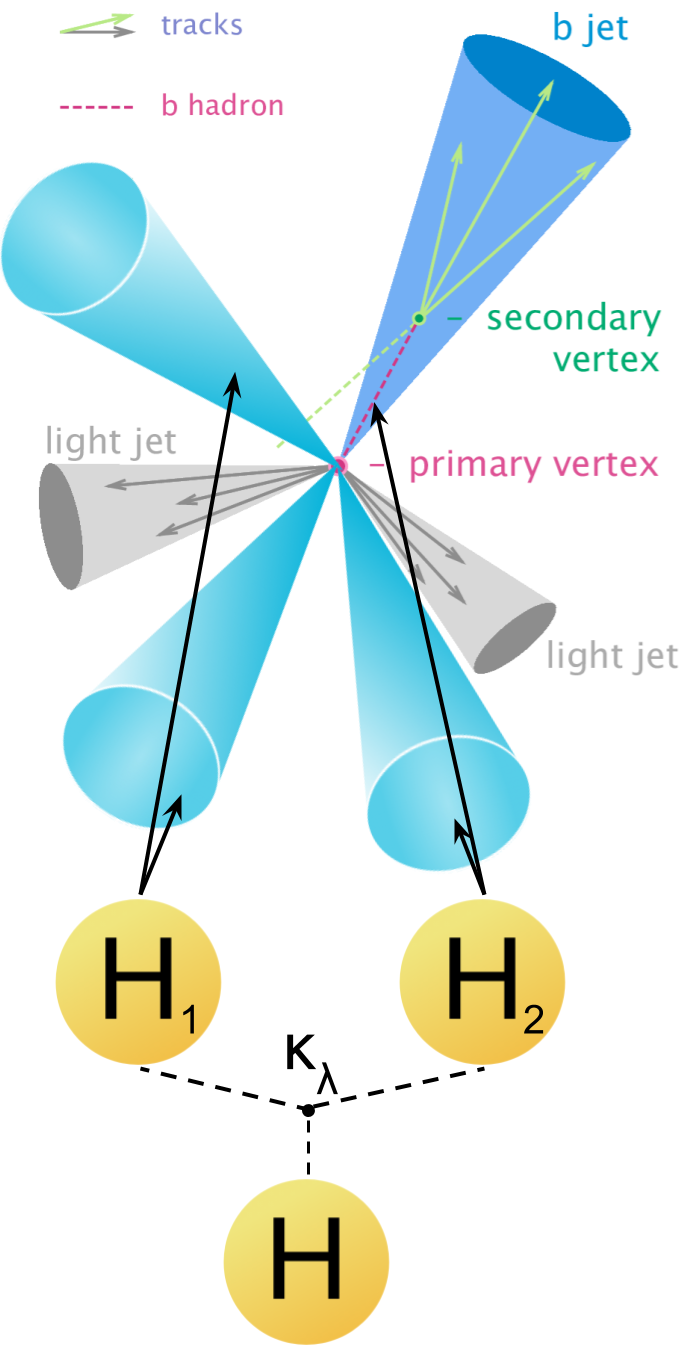
\includegraphics[width=\linewidth]{images/jets_and_pairing.png}
    \end{column}
​  \end{columns}
\end{frame}
}

%%%%%%%%%%%%%%%%%%%%% SLIDE 4
\begin{frame}{$HH$ Backgrounds}
  \begin{itemize}
    \item When looking at $HH$ events, singal = 4 $b$-jets, background = other QCD processes
    \item In 95\% of LHC analyses, backgrounds can be simulated
    (e.g. with GEANT)
    \item But QCD modelling is difficult\\
    (computationally and physics-wise, especially for many-jet events)
    \item Motivates using data for background estimation
    \item But how?
  \end{itemize}
\end{frame}


%%%%%%%%%%%%%%%%%%%%% SLIDE 5
\begin{frame}{Our Project: Background Modelling}
  \begin{itemize}
    \item \alert{Mass plane}: reconstructed $(m_{H_1}, m_{H_2})$ values, $m_{H_1}$ has higher transverse momentum
    \item We expect a peak around $(125, 125)$ (all masses in GeV)
    \item \alert{The Problem}: how to estimate background around peak?\\
    Large source of error ($|\kappa_\lambda| < 7 \to |\kappa_\lambda| < 9$)
    \item Signal Region (SR, in red): blinded to reduce study bias
    \item We want to ``fill in'' the SR
  \end{itemize}
  \centering
  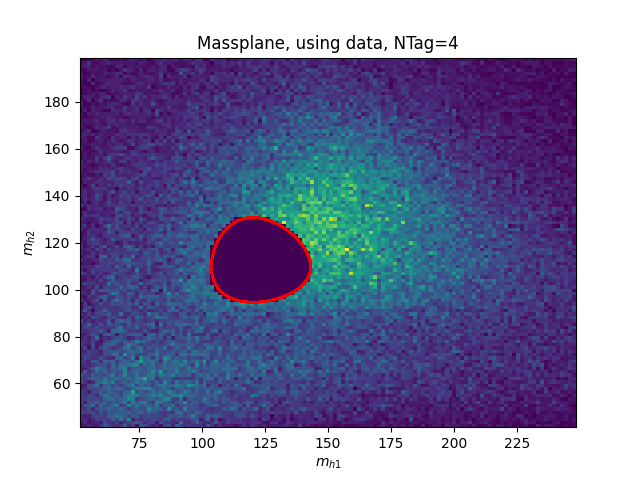
\includegraphics[width=0.35\linewidth, trim = 0 0 0 1.5cm, clip]{images/fullmassplane_4tag_data.png}
\end{frame}

%%%%%%%%%%%%%%%%%%%%% SLIDE 6
\begin{frame}{Current Approach: 2$b$RW}
  \begin{columns}[onlytextwidth]
    \begin{column}{0.6\textwidth}
      \begin{itemize}
        \item All jets are similar to a rough approximation
        \item \alert{2$b$ data}: uses 2 $b$-jets and 2 other jets
        \item Similar to 4$b$ data outside of SR, but no peak
        \item 2$b$RW: derive a scaling (``ReWeighting'') function outside of SR, apply inside
        \item Provides a good first background estimate
        \item Assumes RW function applies in SR, may be false
        \item \alert{This project}: is there a better approach?
      \end{itemize}
    \end{column}
    \begin{column}{0.4\textwidth}
      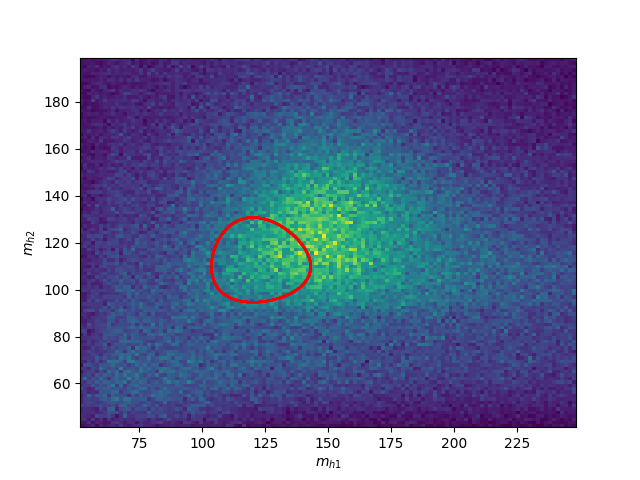
\includegraphics[width=\linewidth]{images/fullmassplane_2tag_data.png}\\
    \end{column}
​  \end{columns}
  \begin{alertblock}{Note}
    Don't forget 2$b$ data is physically different from 4$b$ and 2$b$RW are not \textbf{real} SR values.\\
    2$b$RW is thought to be correct within around $\pm 10\%$.
	\end{alertblock}
\end{frame}

%%%%%%%%%%%%%%%%%%%%% SLIDE 7
{\setbeamertemplate{frame footer}{\vspace{0.2cm}Histogram image from Todd Seiss. Note: this is 4$b$ VR, most plots will use 2$b$RW SR}
\begin{frame}{New Approach: Neural Network}
  \begin{columns}[onlytextwidth]
    \begin{column}{0.6\textwidth}
      \begin{itemize}
        \item Given enough data, neural networks can learn arbitrary functions
        \item Goal: fill in the SR, and reproduce 2$b$RW $\pm 10\%$ using only 4$b$ data
        \item Inputs: $(m_{H_1}, m_{H_2}, m_{HH})$, output: $P(m_{H_1}, m_{H_2})$
        \item Initially: good-looking mass plane predictions,\\
              2$b$RW agreement is not great though
      \end{itemize}
    \end{column}
    \begin{column}{0.4\textwidth}
      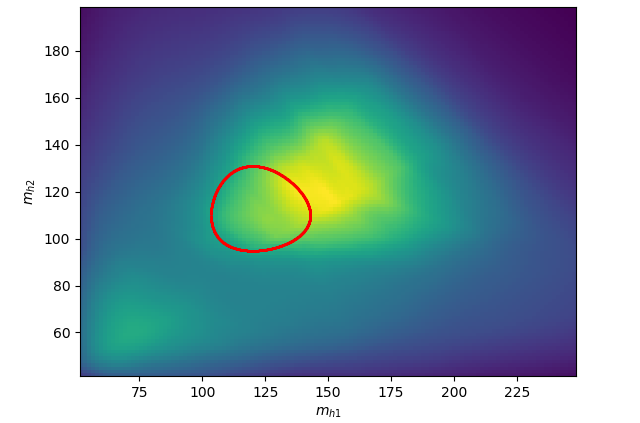
\includegraphics[width=\linewidth]{images/todd_nn_massplane.png}\\
      \hspace{0.3cm}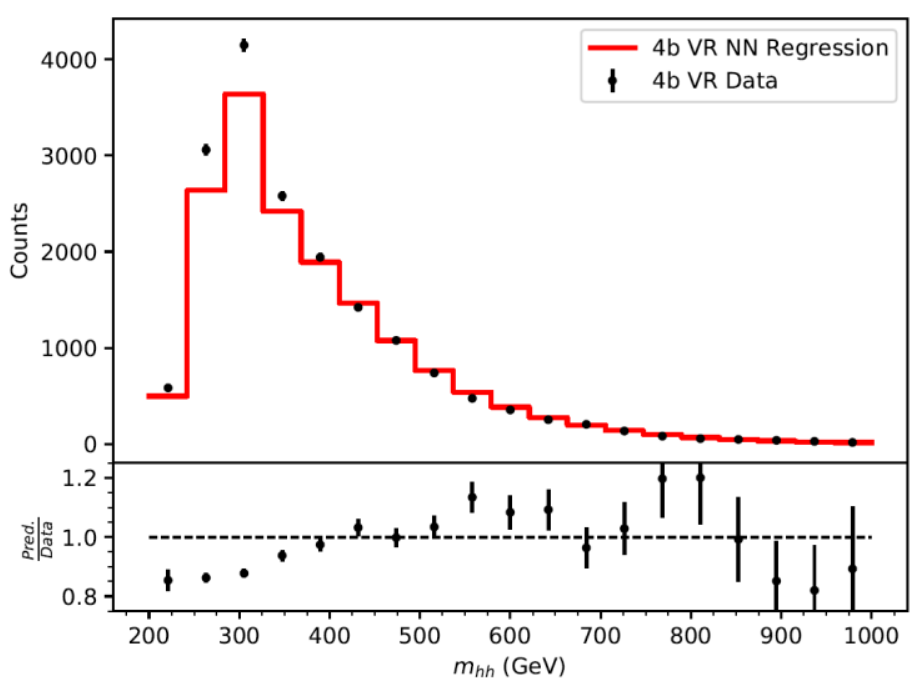
\includegraphics[width=0.9\linewidth]{images/todd_nn_hist.png}\\
    \end{column}
​  \end{columns}
\end{frame}
}

%%%%%%%%%%%%%%%%%%%%% SLIDE 8
\begin{frame}{Neural Network Optimization}
  \begin{columns}[onlytextwidth]
    \begin{column}{0.6\textwidth}
      What if we...
      \begin{itemize}
        \item Further optimize network hyperparameters?
        \item Add more bins?
        \item Add other variables (e.g. more masses, NTag)?
        \item Smooth the data (fit a polynomial, KDE, ...)?
      \end{itemize}
      Overall impression: large improvements unlikely from non-drastic changes in approach
      \begin{itemize}
        \item (note: images are from different models, to show how many of them had similar performance to before)
      \end{itemize}
    \end{column}
    \begin{column}{0.4\textwidth}
      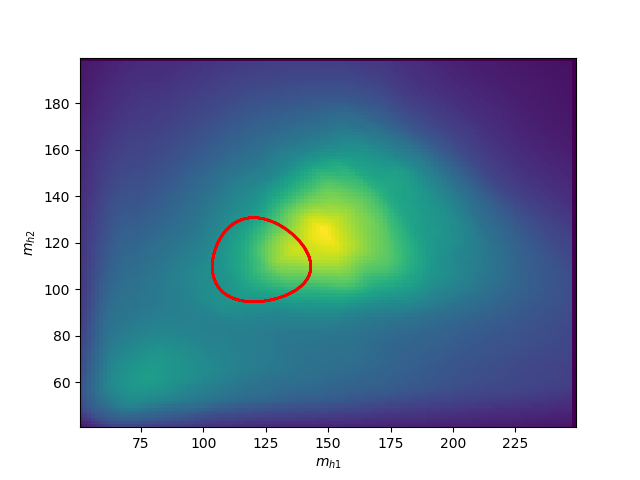
\includegraphics[width=\linewidth]{images/model_20_288_384_416_512_192_30e_25x25_poisson_fullmassplane_4bNN.png}\\
      \hspace{0.3cm}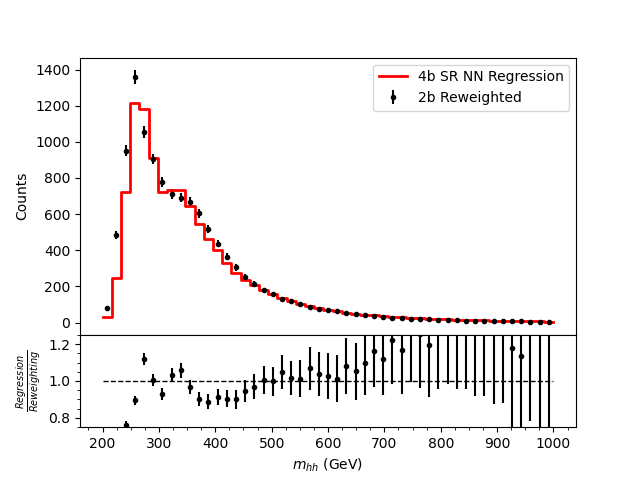
\includegraphics[width=0.9\linewidth]{images/model_2b4b_10505050_30e_25x25_poisson_50mhh_mhhSR.png}\\
    \end{column}
​  \end{columns}
\end{frame}

%%%%%%%%%%%%%%%%%%%%% SLIDE 9
\begin{frame}{New Approach: Gaussian Process Regression}
  \begin{columns}[onlytextwidth]
    \begin{column}{0.6\textwidth}
      \begin{itemize}
        \item Inputs: $m_{H_1}, m_{H_2}$, output: $P(m_{H_1}, m_{H_2})$ 
        \item Also gives estimator variance ($\exists$ assumptions)
        \item Relies on \alert{variogram}
              (ideally could calculate, given finite data must guess)
        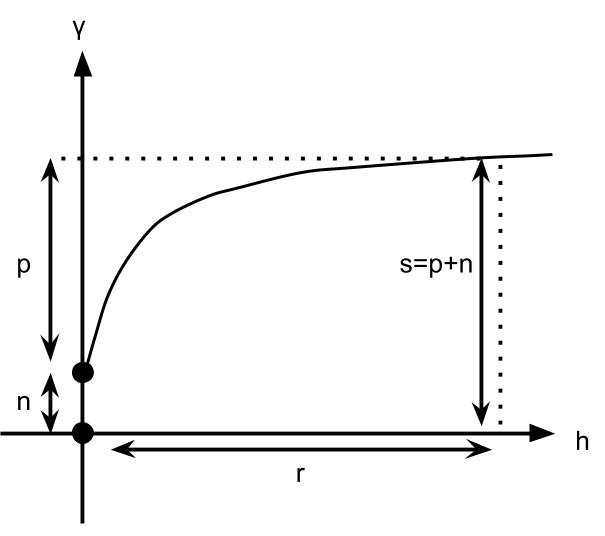
\includegraphics[width=0.5\linewidth]{images/variogram_variables.jpg}\\
        \item Tried a bunch of different ``best-guess'' variograms, e.g. linear and exponential:
      \end{itemize}
    \end{column}
    \begin{column}{0.4\textwidth}
      \phantom{aaaaaa}
      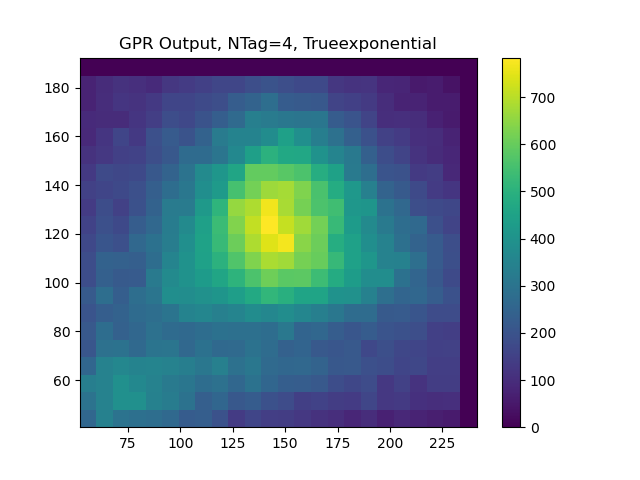
\includegraphics[width=0.8\linewidth, trim=0 0 4cm 1.5cm, clip]{images/kriging_Trueexponential_4b.png}\\
      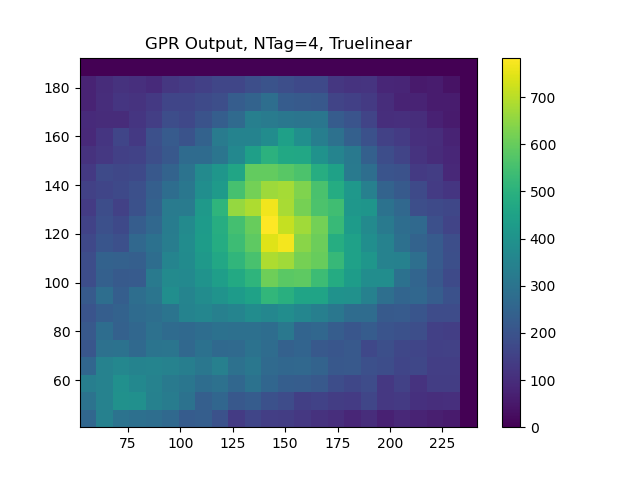
\includegraphics[width=0.8\linewidth, trim=0 0 4cm 1.5cm, clip]{images/kriging_Truelinear_4b.png}\\
    \end{column}
​  \end{columns}
\end{frame}

%%%%%%%%%%%%%%%%%%%%% SLIDE 10
\begin{frame}{GPR Optimization}
  \begin{columns}[onlytextwidth]
    \begin{column}{0.4\textwidth}
      \begin{itemize}
        \item Tested many variograms
        \item Selected low \& flat variance
        \item Best ones still high relative to prediction ($\sim 1 \times$)
        \item Tried 3D GPR, increases computation time too much
      \end{itemize}
      Impressions:
      \begin{itemize}
        \item Good mass plane,\\ less-good histogram
        \item Interesting variances are always so large
        \item Figures: Gaussian variogram ($s=800,r=160,n=10^{-8}$)
      \end{itemize}
    \end{column}
    \begin{column}{0.6\textwidth}
      \includegraphics[width=0.49\linewidth, trim=0 0 0cm 0cm, clip]{images/kriging_Truegaussian{'sill'_ 800, 'range'_ 160, 'nugget'_ 1e-08}_fullmassplane_4b_pred.png}
      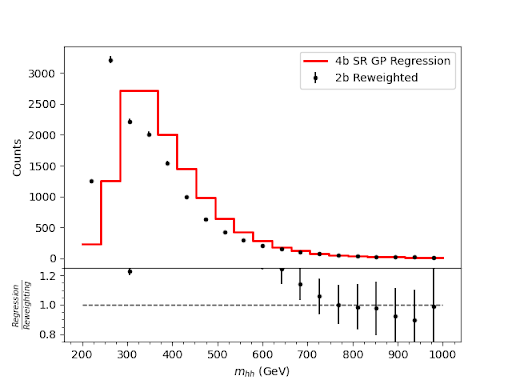
\includegraphics[width=0.49\linewidth, trim=0 0 0cm 0cm, clip]{images/gp_tuned_mhh_histogram.png}
      \includegraphics[width=0.49\linewidth, trim=0 0 0cm 0cm, clip]{images/kriging_variance_Truegaussian{'sill'_ 800, 'range'_ 160, 'nugget'_ 1e-08}_4b.png}
      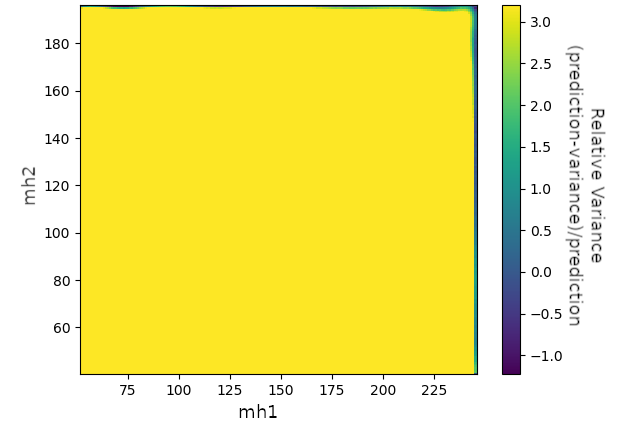
\includegraphics[width=0.49\linewidth, trim=0cm 0cm 0cm 0cm, clip]{images/relative_variance_tuned_gp.png}
    \end{column}
​  \end{columns}
\end{frame}

%%%%%%%%%%%%%%%%%%%%% SLIDE 11
{\setbeamertemplate{frame footer}{Images from Nicole Hartman.}
\begin{frame}{Flow Models}
  \begin{columns}[onlytextwidth]
    \begin{column}{0.6\textwidth}
      \begin{itemize}
        \item The idea of \alert{flows}: build arbitrary function from base function + invertible transformations
        \item \alert{R-NVP} transformations: fast compute times
        \item Benefit: significantly smaller model space, can handle more variables
        \item Code was set up for 2$b$ \alert{pairAGraph} data + figures compare 2$b$ SR prediction vs 2$b$ SR data
        \item With larger models, some nice results are possible (e.g. 5-variable model in figure)
      \end{itemize}
    \end{column}
    \begin{column}{0.4\textwidth}
      \centering
      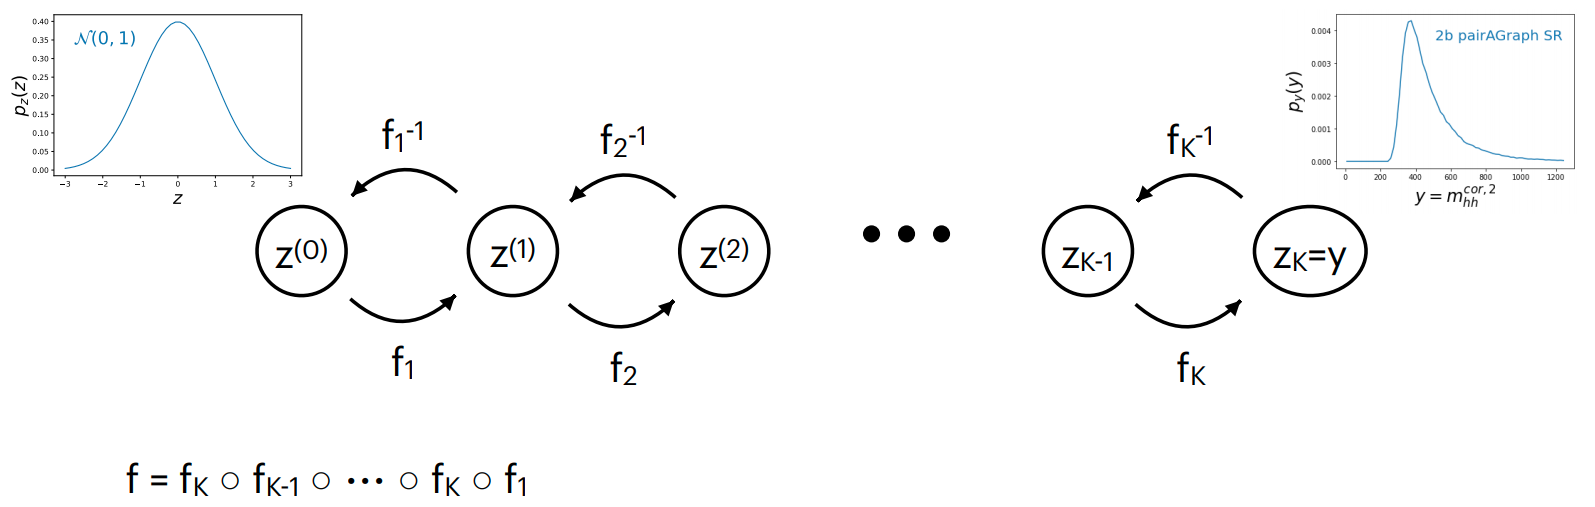
\includegraphics[width=\linewidth, trim=0 0 0cm 0cm, clip]{images/nicole_pres_screenshot.png}
      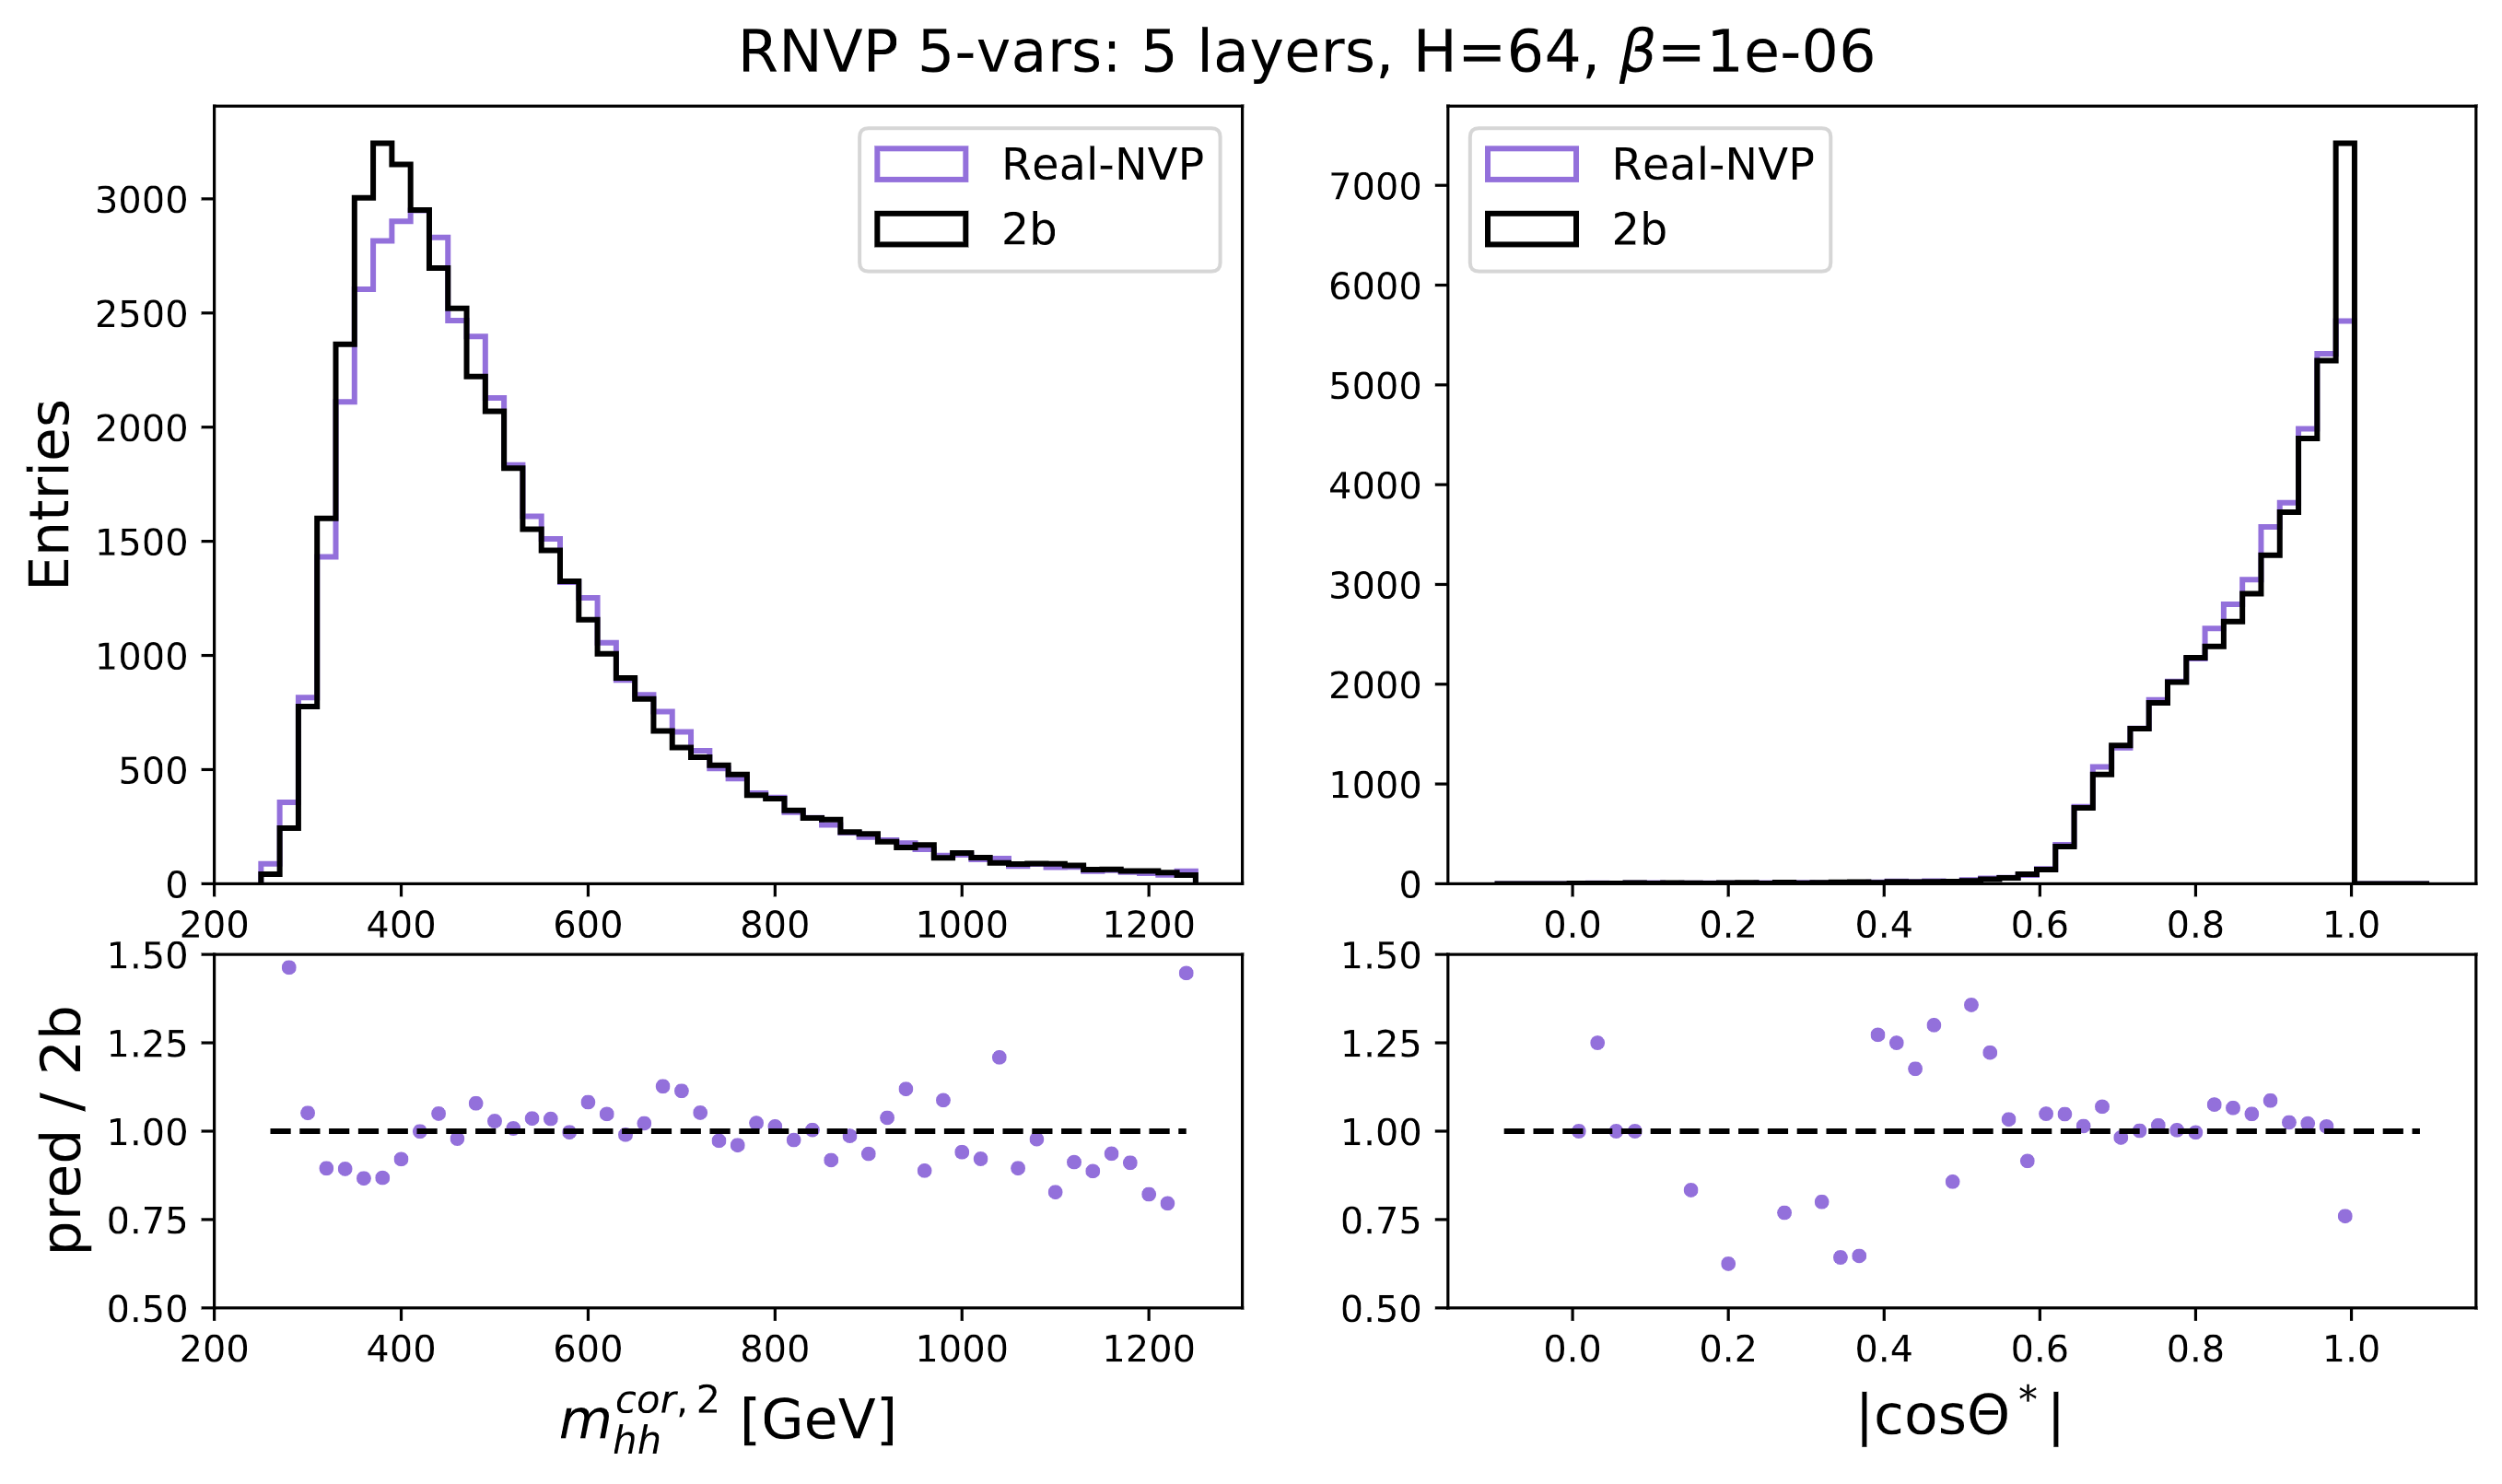
\includegraphics[width=0.7\linewidth, trim=0 0 45cm 4cm, clip]{images/nicole_histogram.png}
    \end{column}
​  \end{columns}
\end{frame}
}
%%%%%%%%%%%%%%%%%%%%% SLIDE 12
\begin{frame}{Comparison of FMs to NNs and GPR}
  \centering
  Use 2$b$ pairAGraph data on previous methods, compare with
  a FM with inputs $(m_{H_1}, m_{H_2})$:\\[1cm]
  \begin{columns}[onlytextwidth]
    \begin{column}{0.33\textwidth}
      \centering
      NN:\\
      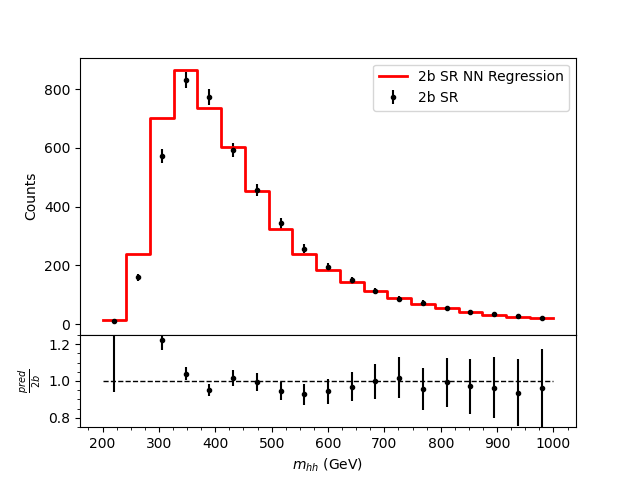
\includegraphics[width=\linewidth, trim=0 0 0cm 0cm, clip]{images/PG_h5_model_2b_10505050_10e_25x25_poisson_20mhh_mhhSR.png}
    \end{column}
    \begin{column}{0.33\textwidth}
      \centering
      GPR:\\
      \includegraphics[width=\linewidth, trim=0 0 0cm 0cm, clip]{images/PG_h5_2d_kriging_Truegaussian{'sill'_ 800, 'range'_ 160, 'nugget'_ 1e-08}_mhhSR.png}
    \end{column}
    \begin{column}{0.33\textwidth}
      \centering
      FM:\\
      \phantom{aaaaaaaaa}\\
      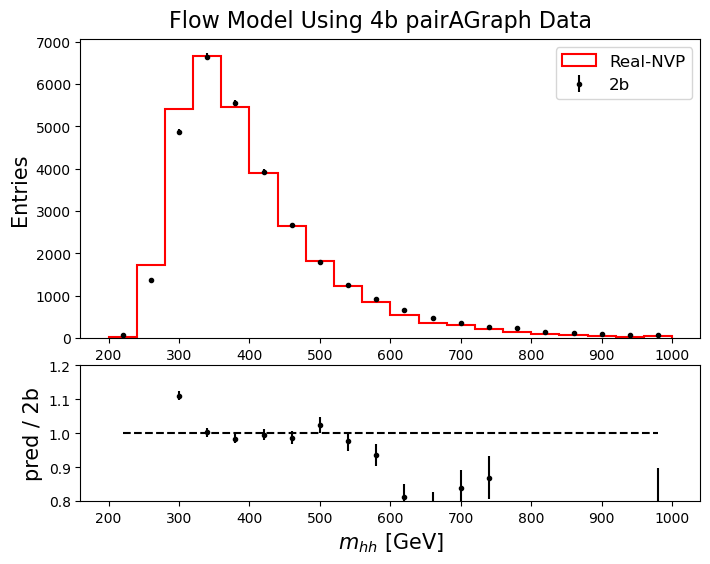
\includegraphics[width=\linewidth, trim=0 0 0cm 1.2cm, clip]{images/flows_m_hh_histogram.png}
    \end{column}
​  \end{columns}
\end{frame}

%%%%%%%%%%%%%%%%%%%%% SLIDE 13
\begin{frame}{Conclusion}
  \begin{itemize}
    \item Direct NN regressions and GPR capture main features of the complicated background
    \item However, the existing 2$b$RW procedure seems to perform better for the moment
    \item Flow models with more variables look promising\\
    (or potentially other similar techniques, e.g. variational auto-encoders)
    %\item Conclude that existing 2$b$RW strategy is currently the best choice
  \end{itemize}
\end{frame}

%%%%%%%%%%%%%%%%%%%%% CLOSER
% set background image to be a massplane or something
{\setbeamercolor{palette primary}{fg=white, bg=mDarkTeal}
\setbeamertemplate{footline}[default]
\begin{frame}[standout, noframenumbering]
  Questions?\\
  Comments?\\
  Any other techniques we should try?
\end{frame}
}

\appendix

%%%%%%%%%%%%%%%%%%%%% BACKUP
\begin{frame}{Backup Slides}
  \centering
  \href{https://docs.google.com/presentation/d/1HImb0b95RuvVrA4HmL7cHfeurqykYyKxsTvzd4683Mw/edit?usp=sharing}{\alert{Link to Google Slides with more details}}
\end{frame}

\end{document}
